%%%%%%%%%%%%%%%%%%%%%%%%%%%%%%%%%%%%%%%%%
%
% (c) 2022 by Jennifer Laaser
%
% This work is licensed under the Creative Commons Attribution-NonCommercial-ShareAlike 4.0 International License. To view a copy of this license, visit http://creativecommons.org/licenses/by-nc-sa/4.0/ or send a letter to Creative Commons, PO Box 1866, Mountain View, CA 94042, USA.
%
% The current source for these materials is accessible on Github: https://github.com/jlaaser/pogil-polymers
%
%%%%%%%%%%%%%%%%%%%%%%%%%%%%%%%%%%%%%%%%%

\renewcommand{\figpath}{content/polymchem/livingpolyms/ideal-living-intro/figs}
\renewcommand{\labelbase}{ideal-living-intro}

\begin{activity}{Ideal, Living Polymerizations}

\begin{instructornotes}
	This activity introduces students to concepts related to ideal, living polymerizations.
	
	After completing this activity, students will be able to:
	\begin{enumerate}
		\item Explain what must be true about the rates of initiation, propagation, and termination in a chain-growth polymerization to achieve polymers with narrow molecular weight distributions 
		\item Describe the molecular weight distributions that are obtained in an ideal, living polymerization and how they compare to those obtained in other polymerizations
	\end{enumerate}
	
	\subsection*{Activity summary:}
	\begin{itemize}
		\item \textbf{Activity type:} Learning Cycle
		\item \textbf{Content goals:} See above
		\item \textbf{Process goals:} %https://pogil.org/uploads/attachments/cj54b5yts006cklx4hh758htf-process-skills-official-pogil-list-2015-original.pdf
			\begin{itemize}
				\item Extrapolation of simulation data to general concepts
				\item Interpretation of mathematical expressions
				\item Oral and written communication of reasoning
			\end{itemize}
		\item \textbf{Duration:} 45 min, including class discussion
		\item \textbf{Instructor preparation required:}
			\begin{itemize}
				\item Model \ref{\labelbase:mdl:poisson} of this activity requires dice (ideally, one die for each student).  If you do not have dice available for use in class, direct students to an online simulator such as https://freeonlinedice.com/
			\end{itemize}
		\item \textbf{Related textbook chapters:}
			\begin{itemize}
				\item \emph{Polymer Chemistry} (Hiemenz \& Lodge), 2nd ed.: sections 4.1 and 4.2
				\item \emph{Introduction to Polymers} (Young \& Lovell), 3rd ed.: concept is briefly introduced in section 4.5; Poisson distribution is introduced in section 5.3.2.4
			\end{itemize}
		%\item \textbf{Facilitation notes:}
		%	\begin{itemize}
		%		\item \dots
		%	\end{itemize}
		\item \textbf{Other notes:}
			\begin{itemize}
				\item As of December 2022, only Model 1 of this activity has been classroom-tested.  Model 2 has been tested with a small group of students, but not a classroom setting - feedback on how to improve Model 2 for classroom use is welcome.
				\item The Hiemenz \& Lodge and Young \& Lovell books use slightly different conventions for where to start counting when determining $N_n$ and $N_w$ for the Poisson distribution.  This activity follows the form given in Hiemenz \& Lodge, in which $PDImath = 1+\frac{\bar v}{(1+\bar v)^2}$ and the dispersity only reduces to $1 + \bar v$ in the large-$\bar v$ limit; Young \& Lovell go directly to $\PDImath = 1+\bar v$.
			\end{itemize}
	\end{itemize}
	
\end{instructornotes}


\begin{model}[What Makes a Polymerization ``Ideal'' and ``Living''?]
	\label{\labelbase:mdl:idealliving}

	Shown below is an illustration of an ``ideal'' chain growth polymerization, in which all chains are initiated at the same time ($t=0$ s) and all grow at the same rate (1 monomer/s):
	    
	    \vspace{6pt}
	    	\centerline{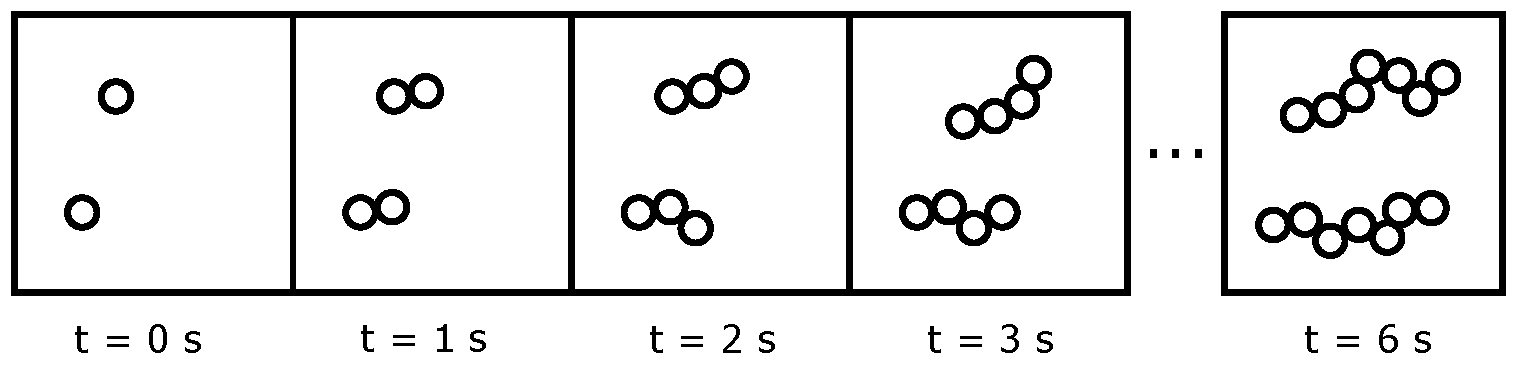
\includegraphics[width=0.8\textwidth]{\figpath/Model1_ideallivingmodel}}
	    	
	    	\emph{Note: for simplicity, unreacted monomers are not shown, but you can assume that there are plenty to allow the reaction to progress.}
	
\end{model}


\begin{ctqs}

	\question What is the dispersity of the polymer sample obtained at the end of the reaction at $t=6$~s?
		
				\emph{Note: it is ok to answer to this question either by doing a calculation or just by using what you know about the meaning of \PDItext.  If you do the former, show your math. If you choose the latter, include a brief explanation of your reasoning.}
			
				\begin{solution}[1.25in]{}
				
					Math answer:
						\begin{align*}
							N_n = \frac{\sum_i i n_i}{\sum_i n_i} = \frac{6\times s}{2} = 6 &&&
							N_w = \frac{\sum_i i^2 n_i}{\sum_i i n_i} = \frac{6^2 \times 2}{6 \times 2} = 6\\
							\PDImath &= \frac{N_w}{N_n} = \frac{6}{6} = 1
						\end{align*}
					
					Conceptual answer:
					
						All of the chain lengths are exactly the same, so the dispersity must be 1.
						
				\end{solution}

	\question Sketch the final distribution of chains you would expect to obtain at $t=6$~s in each of the following alternate cases:

		\begin{enumerate}

			\item Both chains grow at 1 monomer/s but the bottom chain does not start growing until $t=4$~s.
			
				\begin{solution}[0.75in]{}
					\centerline{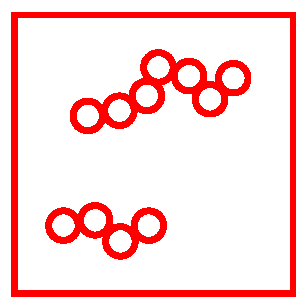
\includegraphics[width=0.5in]{\figpath/Model1_initiation}}(exact answers may vary depending on how students interpret ``starts growing at t=4'')
				
				\end{solution}

			\item Both chains start growing at $t=1$ s, but the bottom chain adds monomers twice as fast as the top chain (i.e. the bottom chain adds 2 monomers/s while the top chain still only adds 1 monomer/s).
			
				\begin{solution}[0.75in]{}
					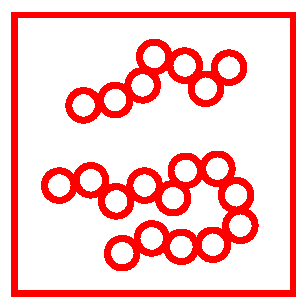
\includegraphics[width=0.75in]{\figpath/Model1_propagation}
				
				\end{solution}

			\item Both chains start growing at $t=1$ s and grow at a rate of 1 monomer/s, but the top chain stops growing after t=4~s.
			
				\begin{solution}[0.75in]{}
					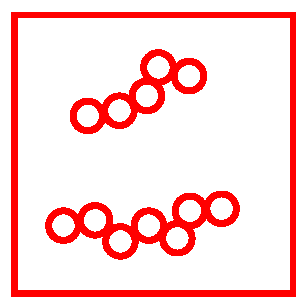
\includegraphics[width=0.75in]{\figpath/Model1_termination} 
				
				\end{solution}
				
		\end{enumerate}
		
	\question Based on your group's answers to the previous question, write a short paragraph summarizing what needs to be true about the initiation, propagation, and termination processes in a chain-growth polymerization if you want to obtain a low-dispersity polymer.
	
		\begin{solution}[2in]{}
			To obtain a low-dispersity polymer, the following conditions must be met: first, all of the chains must initiate at the same time.  Second, all of the chains must grow at the same rate.  And third, none of the chains can terminate early (or, all of them must terminate at the same time.)
		\end{solution}

\end{ctqs}

\begin{infobox}

	Chain-growth polymerizations that proceed in the absence of irreversible termination and chain-transfer reactions are termed \emph{living} polymerizations.
	
	Chain-growth polymerizations in which the chains additionally all start growing at the same time \emph{and} all grow at the same rate are termed \emph{ideal} living polymerizations.

\end{infobox}

\begin{ctqs}

	\question Is free-radical polymerization an ideal, living polymerization?  Why or why not?  Explain your group's reasoning in 2-3 complete sentences.
	
		\begin{solution}[2in]{}
			No, free-radical polymerization is not an ideal, living polymerization.  Most importantly, the propagating chains can terminate at any point during the reaction if they encounter another chain with an active radical on the end, and that termination process is permanent, so free radical polymerization does NOT proceed in the absence of irreversible termination.  Additionally, however, initiation usually takes place over some period of time determined by the initiator's decomposition rate, so the chains also do not all initiate at the same time (even if the active radicals do, generally, grow at about the same rate once they are formed).
		\end{solution}

\end{ctqs}

%\clearpage
\begin{model}[Chain Length Distributions in Ideal, Living Polymerizations]
	\label{\labelbase:mdl:poisson}

		In an ideal, living polymerization, the monomers end up being randomly distributed between the chains.  Simulate this process by doing the following:
		\begin{enumerate}
			\item Obtain a cup of dice from your instructor, and distribute one die to each student in your group.
			\item Roll your die, and add a ``monomer'' to the chain corresponding to the number on the die by drawing a circle at the end of the chain.
			\item Repeat step 2 until you have added a total of 20 monomers to the chains.  Do this process individually - each person in your group should generate their own distribution of chains.
		\end{enumerate}
		
		\vspace{-18pt}
		\begin{solution}[2.5in]{\centerline{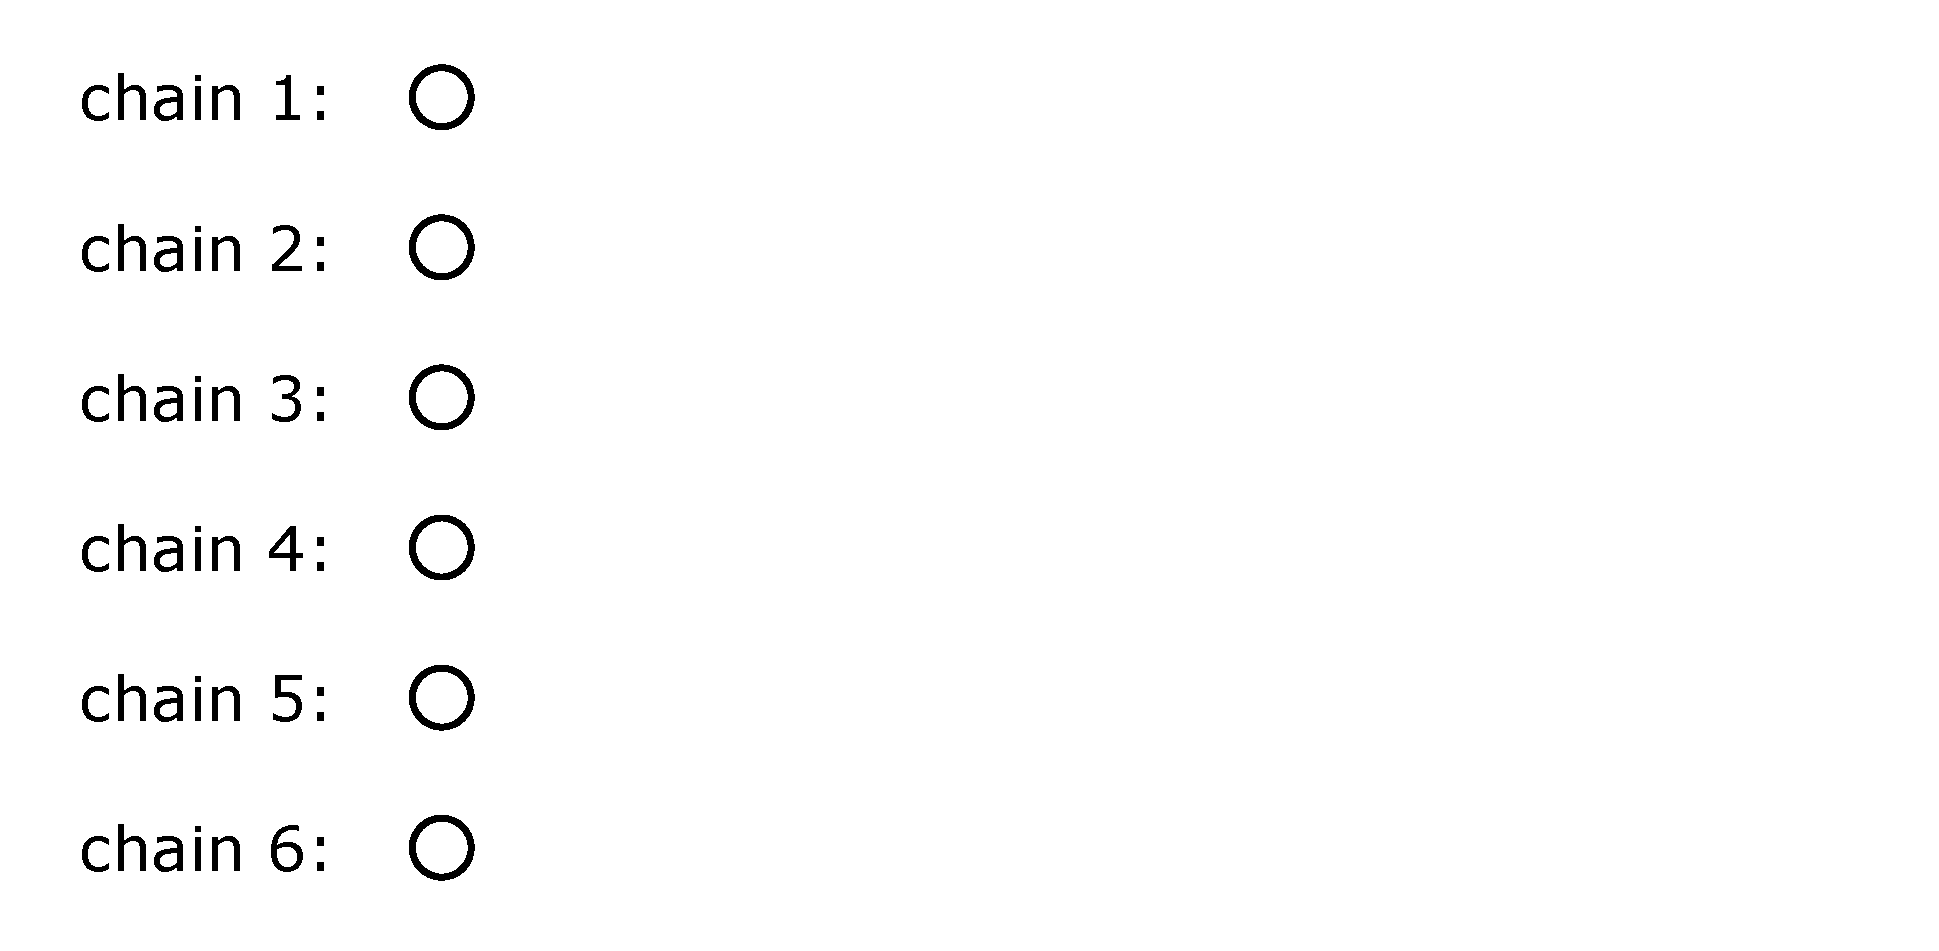
\includegraphics[width=0.8\textwidth]{\figpath/Model2_blank}}}\centerline{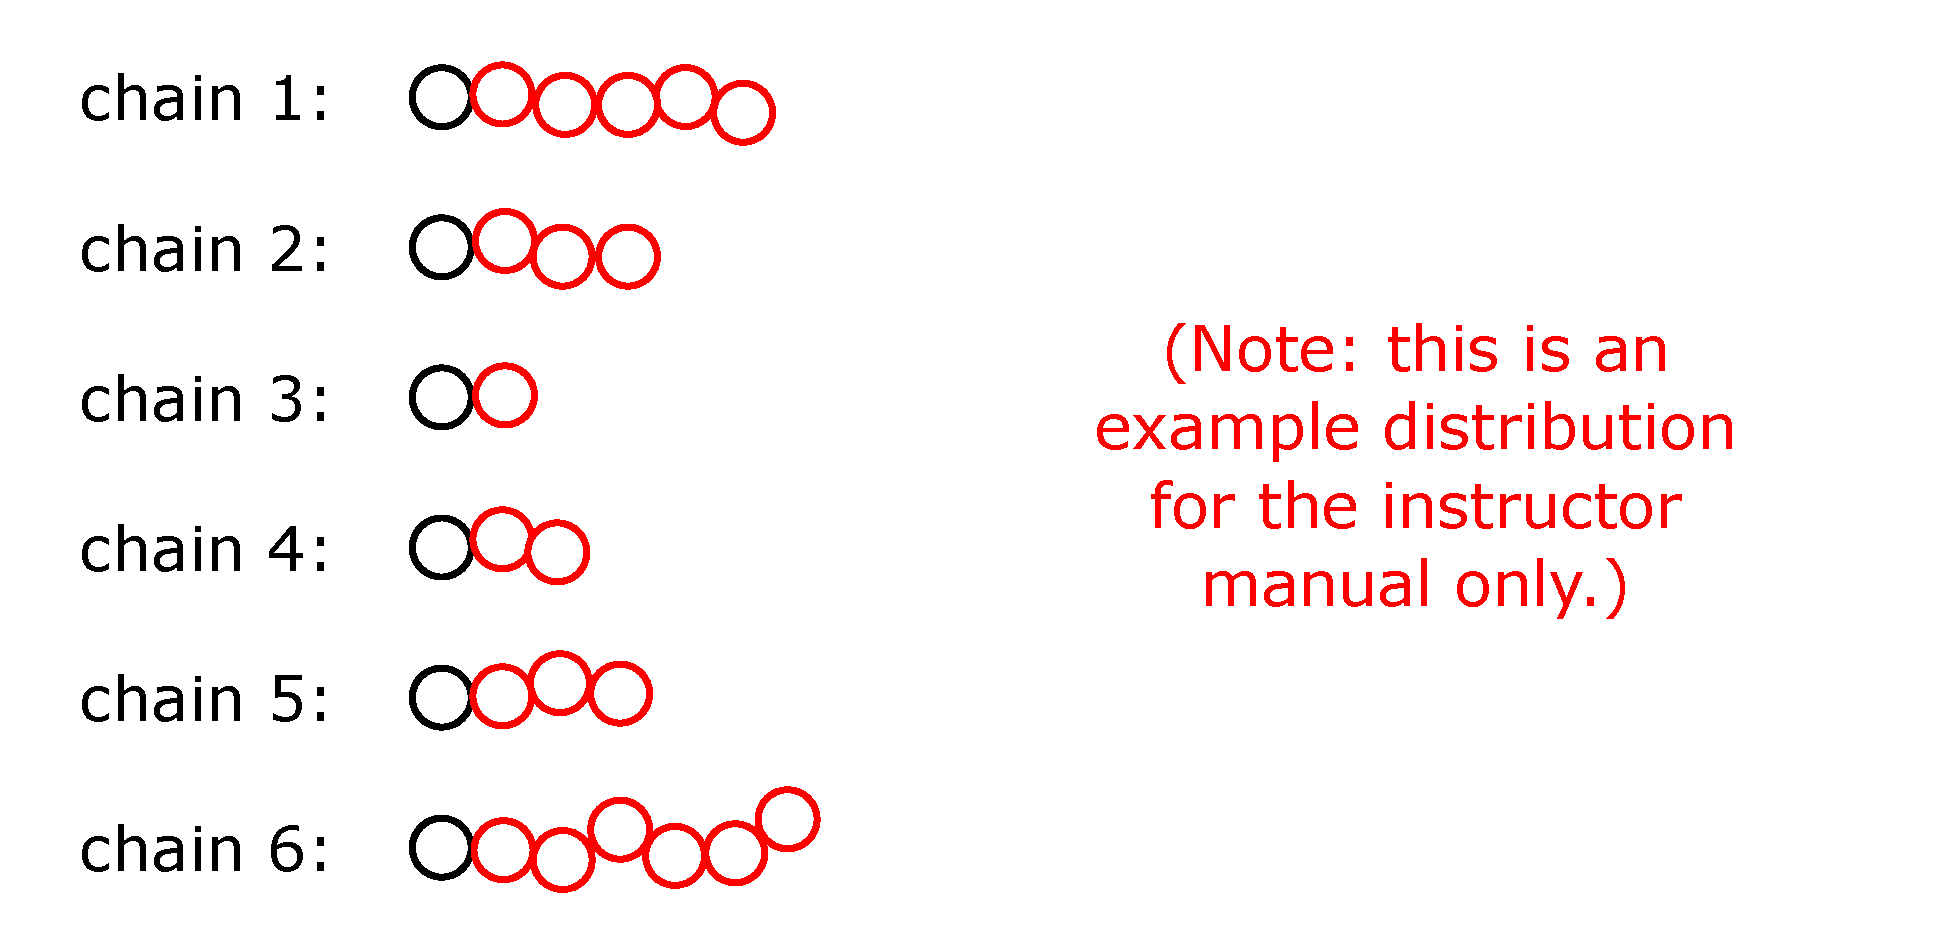
\includegraphics[width=0.8\textwidth]{\figpath/Model2_examplesoln}}\end{solution} %this is inelegant but the only way I can get the different graphics to display here...
	
\end{model}

\begin{ctqs}
	
	\question For the distribution you generated in this simulation, calculate... \label{\labelbase:ctq:simulationcalcs}
	
		\begin{enumerate}
			\item The number-average degree of polymerization:
			
				\emph{(Hint: you will find it useful to recall that $N_n = \frac{\sum_i i n_i}{\sum_i n_i}$, where $i$ is a chain length and $n_i$ is the number of chains with that length.)}
			
				\begin{solution}[2in]{}
					For the example distribution shown above,
					\begin{equation*}
						N_n = \frac{5\cdot 1 + 3\cdot 1 + 1\cdot 1 + 2\cdot 1 + 3\cdot 1 + 6\cdot 1}{1+1+1+1+1+1} = \frac{20}{6}=3.333
					\end{equation*}
					Note: students should ideally only count the monomers they added, not the ``initiator'' circle that was already shown in the model, but the activity will work either way.
				\end{solution}
			
			\clearpage
			\item The weight-average degree of polymerization \emph{(Similarly, recall that $N_w= \frac{\sum_i i^2 n_i}{\sum_i i n_i}$)}:
			
				\begin{solution}[1.25in]{}
					For the example distribution shown above,
					\begin{equation*}
						N_n = \frac{5^2\cdot 1 + 3^2\cdot 1 + 1^2\cdot 1 + 2^2\cdot 1 + 3^2\cdot 1 + 6^2\cdot 1}{5\cdot 1 + 3\cdot 1 + 1\cdot 1 + 2\cdot 1 + 3\cdot 1 + 6\cdot 1} = \frac{84}{20}=4.2
					\end{equation*}
				\end{solution}
			
			\item The dispersity of the distribution, $\PDImath = \frac{N_w}{N_n}$:
			
				\begin{solution}[0.75in]{}
					For the example distribution shown above,
					\begin{equation*}
						\PDImath = \frac{4.2}{3.333} = 1.26
					\end{equation*}
				\end{solution}
			
		\end{enumerate}
		
	\question Your group also could also have worked together and contributed all of your dice rolls to one set of chains.  Determine the lengths of the chains you would have ended up with in this case (i.e. add up the length of everyone's ``chain 1'' to get the length of the long ``chain 1'' you would have obtained, and then do the same for chains 2, 3, etc.) and write them down below.
		
		\begin{center}
			\renewcommand{\arraystretch}{2.5}
			\begin{tabular}{|l|c|l|c|l|c|}
				\hline
				Chain 1: & ~~~~~~~\answer{17}~~~~~~~ & Chain 2: & ~~~~~~~\answer{13}~~~~~~~  & Chain 3: & ~~~~~~~\answer{16}~~~~~~~  \\\hline
				Chain 4: & ~~~~~~~\answer{9}~~~~~~~ & Chain 5: & ~~~~~~~\answer{12}~~~~~~~  & Chain 6: & ~~~~~~~\answer{13}~~~~~~~  \\\hline
			\end{tabular}
		\end{center}
		
	\question Calculate $N_n$, $N_w$, and $\PDImath$ for this new, longer distribution of chains, and comment on how the values compare to your the numbers you came up with in CTQ \ref{\labelbase:ctq:simulationcalcs}.
			
		\begin{solution}[3in]{}
			For the above distribution, which was obtained from 80 dice rolls (4 students combining their individual data),
			\begin{align*}
				N_n &= \frac{17+13+16+9+12+13}{6} = \frac{80}{6} = 13.33\\
				N_w &= \frac{17^2+13^2+16^2+9^2+1^22+13^2}{17+13+16+9+12+13} = \frac{1108}{80} = 13.85\\
				\PDImath &= \frac{N_w}{N_n} = \frac{13.85}{13.33} = 1.04
			\end{align*}
			The number-average and weight-average degrees of polymerization have increased, but the dispersity has decreased.
			
			(Note: occasionally, a student will find that the summed distribution has a higher \PDItext\ than the distribution they obtained from their individual dice rolls.  When this occurs, ask them to consider what trend is most prevalent \emph{across their group}.)
		\end{solution}
	
\end{ctqs}

\begin{infobox}

	In the limit of many monomers and many chains, the distribution of chain lengths in an ideal, living polymerization follows the \emph{Poisson distribution},
	\begin{equation*}
		x_i = \frac{\bar v^{i-1}e^{-\bar v}}{(i-1)!}
	\end{equation*}
	where $\bar v$ is the kinetic chain length, or the number of monomers that have been incorporated into chains divided by the total number of chains.
	
	It is possible to show that the dispersity of this distribution is
	\begin{equation*}
		\PDImath = 1+\frac{\bar v}{(1+\bar v)^2}
	\end{equation*}

	\label{\labelbase:infobox:poisson}

\end{infobox}

\begin{ctqs}

	\question Calculate the dispersity expected for each of the following kinetic chain lengths: \label{\labelbase:ctq:poissondispersities}
	
		\begin{enumerate}
		
			\item $\bar v = 10$:
			
				\begin{solution}[0.25in]{}
					\begin{equation*}
						\PDImath = 1+\frac{10}{(1+10)^2} = 1.083
					\end{equation*}
				\end{solution}
			
			\item $\bar v = 100$:
			
				\begin{solution}[0.25in]{}
					\begin{equation*}
						\PDImath = 1+\frac{100}{(1+100)^2} = 1.0098
					\end{equation*}
				\end{solution}
			
			\item $\bar v = 1000$:
			
				\begin{solution}[0.25in]{}
					\begin{equation*}
						\PDImath = 1+\frac{1000}{(1+1000)^2} = 1.00099
					\end{equation*}
				\end{solution}
			
		\end{enumerate}
		
	\question One of your classmates looks at the expression for $\PDImath$ given above and says, \emph{``Oh!  When the chains get really long, the dispersity in an ideal living polymerization is essentially just $\PDImath = 1+\frac{1}{N_n}$.''}
	
		Is your classmate correct?  Explain your group's reasoning in 2-3 complete sentences.
		
		\begin{solution}[2in]{}
			Yes, your classmate is correct.  First, because the kinetic chain length is the number of monomers that have been incorporated into chains divided by the total number of chains, the kinetic chain length is equal to the number-average degree of polymerization of the polymers (at least, as long as we do not do anything to intentionally couple the chains at the end of the reaction).  This lets us rewrite
	\begin{equation*}
		\PDImath = 1+\frac{N_n}{(1+N_n)^2}
	\end{equation*}
			Second, when the chains are long, $N_n$ is large and $1+N_n \approx N_n$.  This lets us simplify the expression to 
	\begin{equation*}
		\PDImath \approx 1+\frac{N_n}{N_n^2} = 1+\frac{1}{N_n}
	\end{equation*}
	exactly as your classmate claimed. Note that this is also roughly consistent with the calculations above - it is quite a good approximation even for $N_n=10$!
		\end{solution}
		
	\clearpage
	\question Based on this expression, what is the limiting value of the dispersity when the chains become infinitely long?
		
		\begin{solution}[0.5in]{}
			As $\bar v \to \infty$, $\PDImath \to 1$.
		\end{solution}
	
	\question Finally, how does the value calculated in the previous question compare to the limiting values you expect for (a) step-growth polymerizations, and (b) free-radical polymerizations?  Comment briefly on why ideal, living polymerizations might be preferred if you are trying to make a polymer with a well-defined molecular weight.
		
		\begin{solution}[1.5in]{}
			The limiting value of the dispersity for step-growth polymerizations is 2, while that for free-radical polymerizations is either 1.5 or 2 depending on the mechanism of termination (combination or disproportionation, respectively).  The dispersity obtained in the infinite molecular weight limit for an ideal living polymerization is, by comparison, much lower - as we learned above, ideal, living polymerizations can theoretically produce dispersities less than 1.1 even for very short chains,  and the dispersities decrease with increasing molecular weight.  This means that for an application requiring a polymer with a well-defined molecular weight, ideal living polymerizations will be a much better way to realize that goal than either step-growth or free-radical polymerizations.
		\end{solution}
	
\end{ctqs}



\begin{exercises}

	\exercise Plot the Poisson distribution (page \pageref{\labelbase:infobox:poisson}) for $\bar v = 10$, 20, and 50, and 100.  Comment on how the plots compare.  Are you at all surprised by their relative shapes, given what you learned about how dispersity changes with chain length in this activity?  Propose a reason for any discrepancies you notice.
	
		\begin{solution}{}
			\centerline{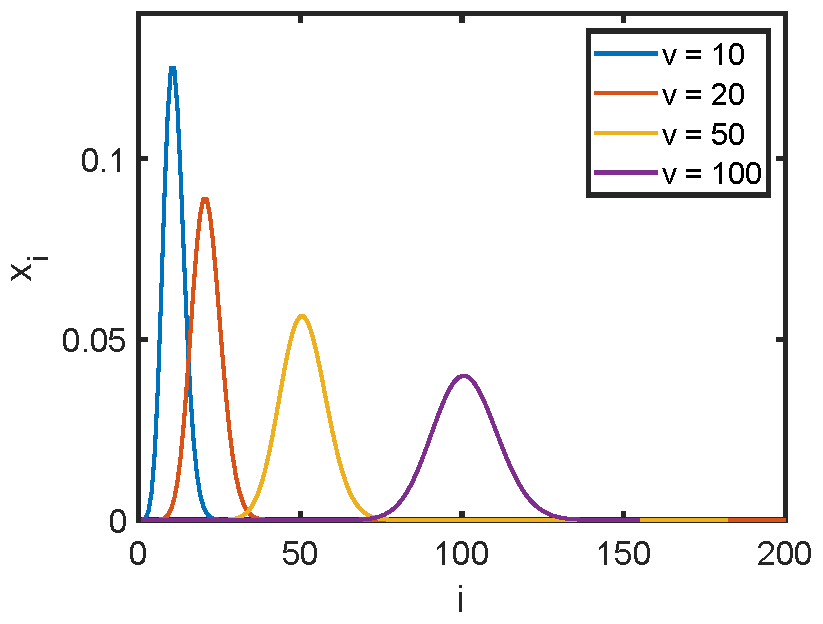
\includegraphics[width=0.5\textwidth]{\figpath/Exc1_poissonplots.pdf}}
			
			The distributions broaden as the average chain length increases, which students may find a little counterintuitive given that the dispersity of the Poisson distribution \emph{decreases} as the chain length increases.  The key, however, is to remember that dispersity is related to the \emph{ratio} of the standard deviation of the distribution to the average; even though the distributions (and their standard deviations) broaden as the chain length increases, the \emph{ratio} of the standard deviation to the average value decreases.  A simple way to see this is to look at how far the tails of the distribution extend toward zero - for $\bar v = 10$, the tails reach all the way to 0, while for $\bar v = 100$ the tails appear to end much earlier.
		\end{solution}
	
	%\exercise Plot the Poisson distribution for an ideal, living polymerization with $\bar v = 100$ on the same axes as plots of the corresponding distributions for (a) a free-radical polymerization that terminates by disproportionation and (b) a free-radical polymerization that terminates by combination, both with the same number-average molecular weight.  Comment briefly on how the shapes of the curves compare.
		% note: leaving this one out for now - don't yet have an activity on MWDs for free-radical, so students don't have the equations to do this correctly
	
\end{exercises}




%\begin{problems}
%
%	\problem First exercise
%	\problem Second exercise
%	
%\end{problems}


	
\end{activity}